%%%%%%%%%%%%%%%%%%%%%%%%%%%%%%%%%%%%%%%%%
% Short Sectioned Assignment
% LaTeX Template
% Version 1.0 (5/5/12)
%
% This template has been downloaded from:
% http://www.LaTeXTemplates.com
%
% Original author:
% Frits Wenneker (http://www.howtotex.com)
%
% License:
% CC BY-NC-SA 3.0 (http://creativecommons.org/licenses/by-nc-sa/3.0/)
%
%%%%%%%%%%%%%%%%%%%%%%%%%%%%%%%%%%%%%%%%%

%----------------------------------------------------------------------------------------
%	PACKAGES AND OTHER DOCUMENT CONFIGURATIONS
%----------------------------------------------------------------------------------------

\documentclass[paper=a4, fontsize=11pt]{scrartcl} % A4 paper and 11pt font size

\usepackage[T1]{fontenc} % Use 8-bit encoding that has 256 glyphs
%\usepackage{fourier} % Use the Adobe Utopia font for the document - comment this line to return to the LaTeX default
\usepackage[english]{babel} % English language/hyphenation
\usepackage{amsmath,amsfonts,amsthm} % Math packages

\usepackage{lipsum} % Used for inserting dummy 'Lorem ipsum' text into the template

\usepackage{graphicx}
\usepackage{caption}
\usepackage{subcaption}

\usepackage{sectsty} % Allows customizing section commands
\allsectionsfont{\centering \normalfont\scshape} % Make all sections centered, the default font and small caps

\usepackage{fancyhdr} % Custom headers and footers
\pagestyle{fancyplain} % Makes all pages in the document conform to the custom headers and footers
\fancyhead{} % No page header - if you want one, create it in the same way as the footers below
\fancyfoot[L]{} % Empty left footer
\fancyfoot[C]{} % Empty center footer
\fancyfoot[R]{\thepage} % Page numbering for right footer
\renewcommand{\headrulewidth}{0pt} % Remove header underlines
\renewcommand{\footrulewidth}{0pt} % Remove footer underlines
\setlength{\headheight}{13.6pt} % Customize the height of the header

\numberwithin{equation}{section} % Number equations within sections (i.e. 1.1, 1.2, 2.1, 2.2 instead of 1, 2, 3, 4)
\numberwithin{figure}{section} % Number figures within sections (i.e. 1.1, 1.2, 2.1, 2.2 instead of 1, 2, 3, 4)
\numberwithin{table}{section} % Number tables within sections (i.e. 1.1, 1.2, 2.1, 2.2 instead of 1, 2, 3, 4)

\setlength\parindent{0pt} % Removes all indentation from paragraphs - comment this line for an assignment with lots of text

%----------------------------------------------------------------------------------------
%	TITLE SECTION
%----------------------------------------------------------------------------------------

\newcommand{\horrule}[1]{\rule{\linewidth}{#1}} % Create horizontal rule command with 1 argument of height

\title{	
\normalfont \normalsize 
\textsc{ETH Zurich, D-INFK} \\ [25pt] % Your university, school and/or department name(s)
\horrule{0.5pt} \\[0.4cm] % Thin top horizontal rule
\huge Computer Vision Exercise 11: Segmentation \\ % The assignment title
\horrule{2pt} \\[0.5cm] % Thick bottom horizontal rule
}

\author{Igor Pesic} % Your name

\date{\normalsize\today} % Today's date or a custom date

\begin{document}

\maketitle % Print the title


\section{Preprocessing}
Preprocessing is done with Gaussian filter with $\sigma=5$ and filter size $5\times5$. The results are shown in Figures \ref{fig:cow} and \ref{fig:zebra}.

\begin{figure}
\centering
\begin{subfigure}{.5\textwidth}
  \centering
  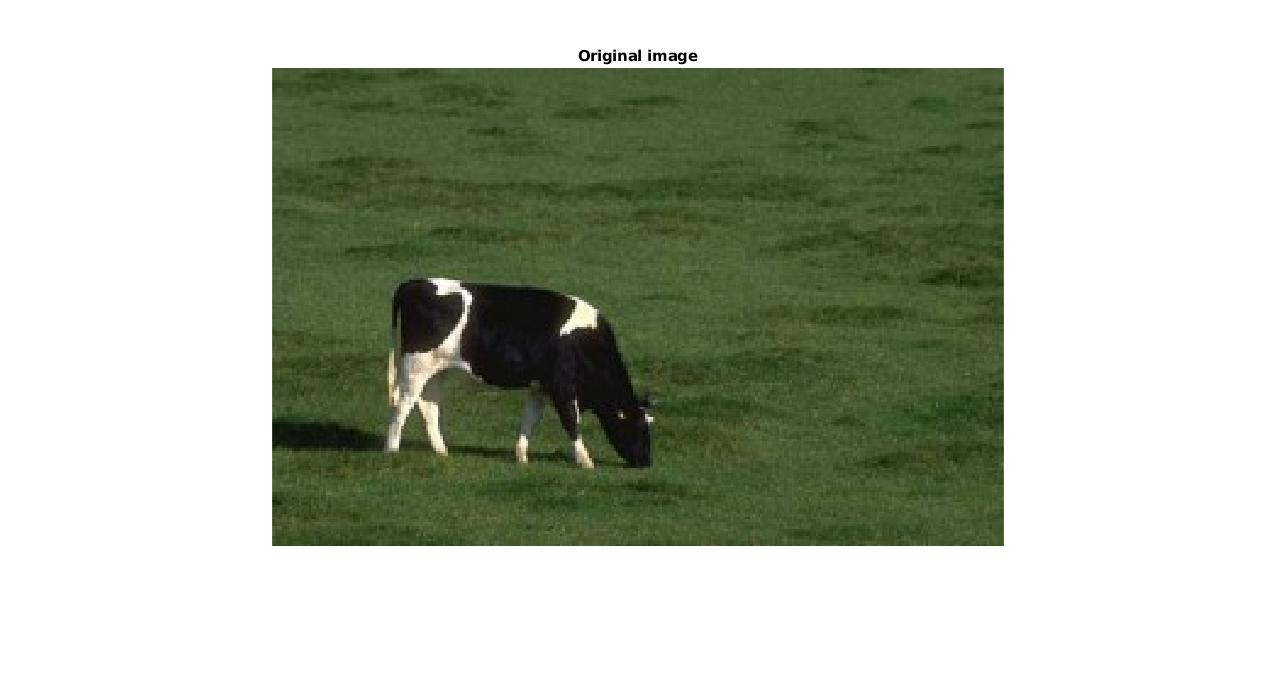
\includegraphics[width=\linewidth]{cow/orig.jpg}
  \caption{Original}
\end{subfigure}%
\begin{subfigure}{.5\textwidth}
  \centering
  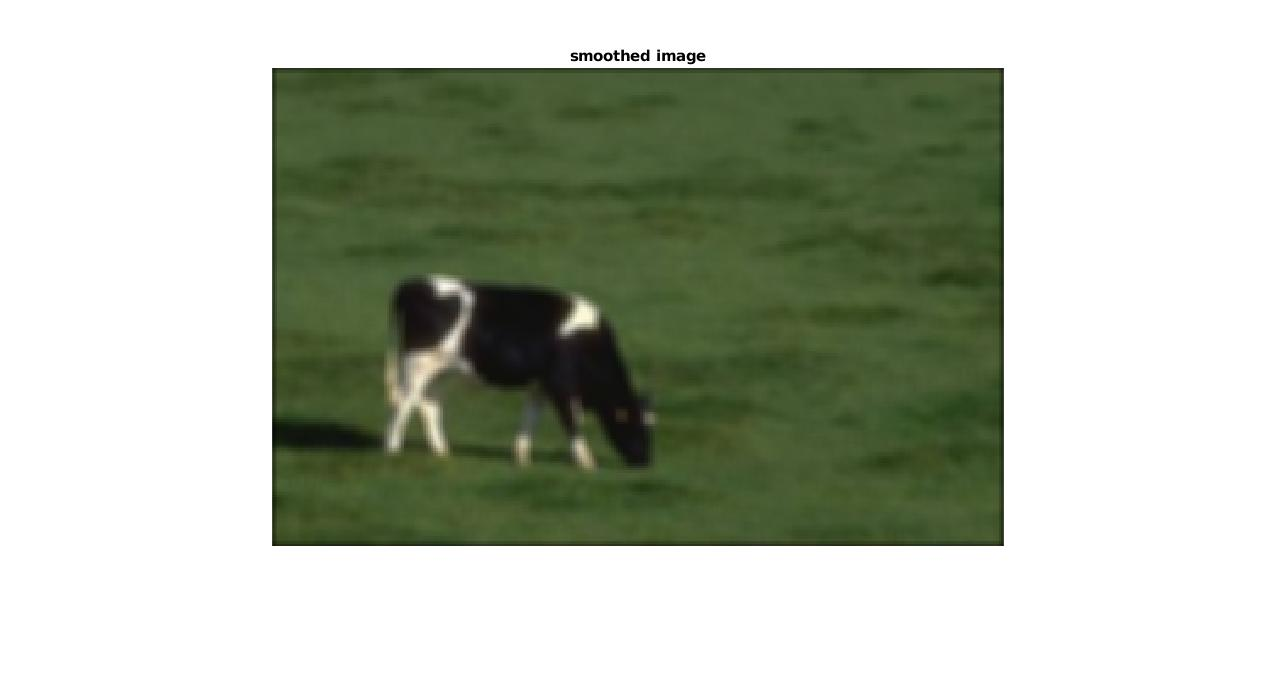
\includegraphics[width=\linewidth]{cow/smooth.jpg}
  \caption{Smooth}
\end{subfigure}
\caption{Cow image after preprocessing}
\label{fig:cow}
\end{figure}

\begin{figure}
\centering
\begin{subfigure}{.5\textwidth}
  \centering
  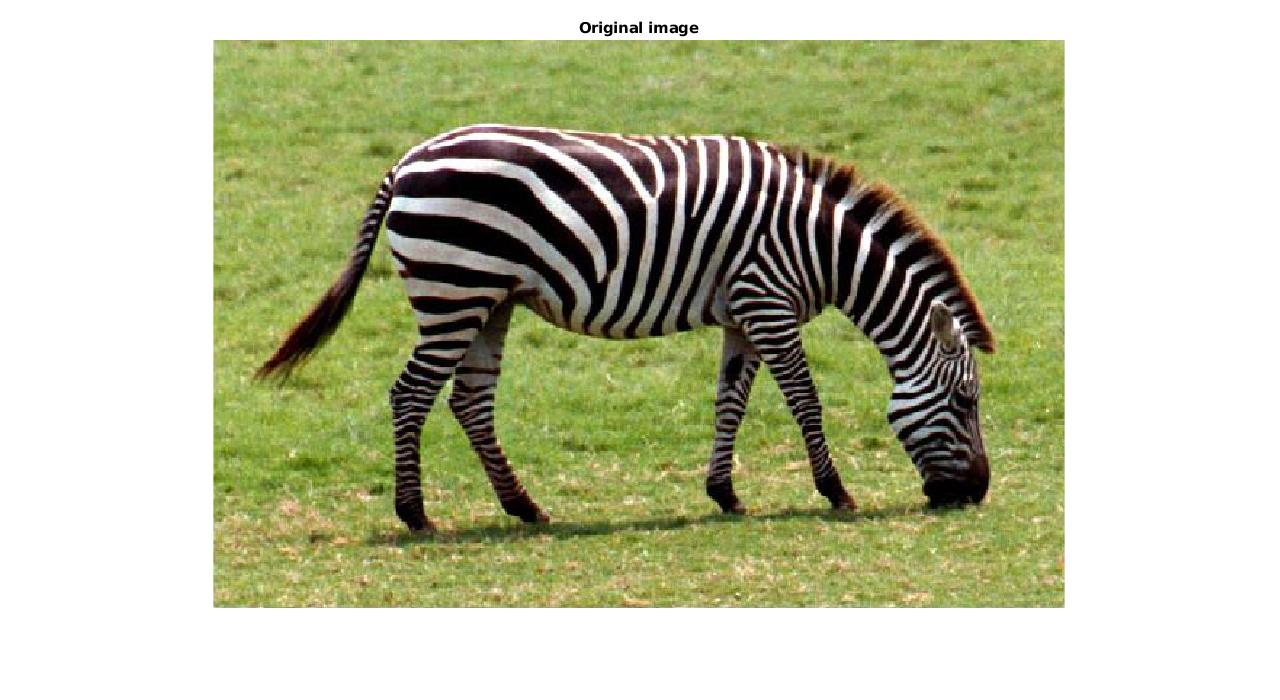
\includegraphics[width=\linewidth]{zebra/orig.jpg}
  \caption{Original}
\end{subfigure}%
\begin{subfigure}{.5\textwidth}
  \centering
  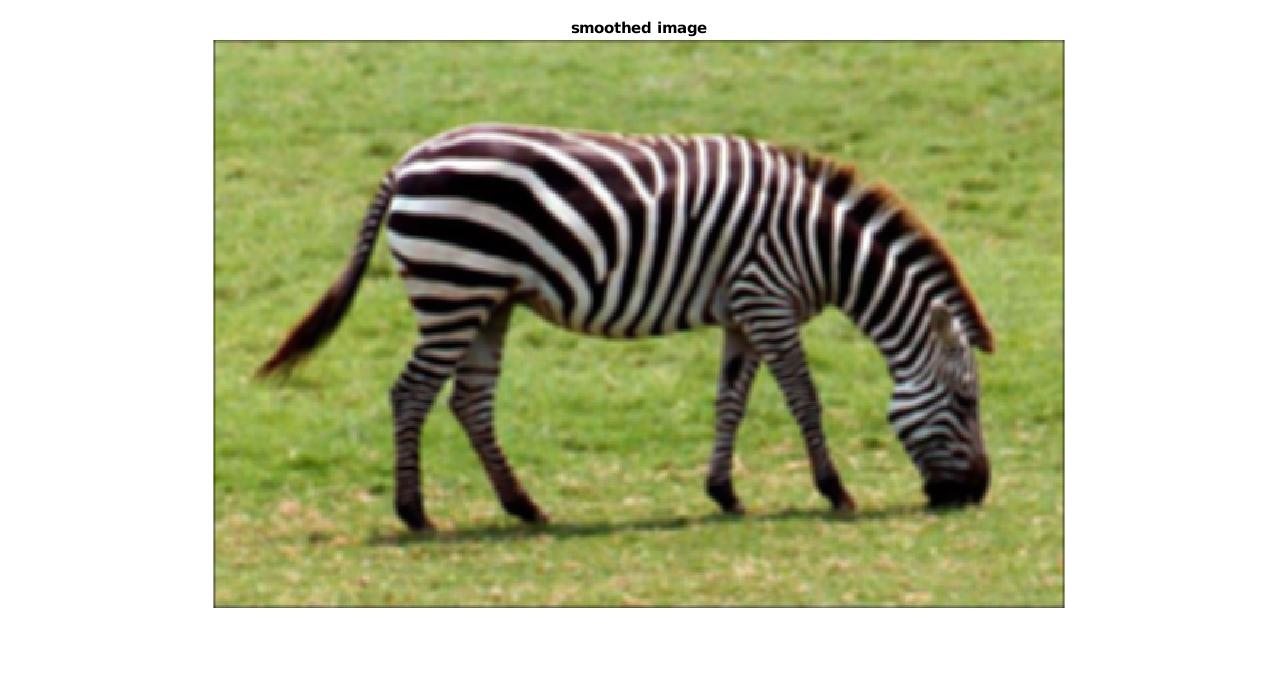
\includegraphics[width=\linewidth]{zebra/smooth.jpg}
  \caption{Smooth}
\end{subfigure}
\caption{Zebra image after preprocessing}
\label{fig:zebra}
\end{figure}


\section{Mean-Shift Segmentation}

Mean-shift algorithm is implemented as described in the exercise sheet and the slides. Since my implementation is very slow, I have run it with rescaled zebra image with scale factor of 0.5 and the original sized cow image. For both images I have chosen $radius=10$. I have also normalized the pixels to 0 mean and $\sqrt{3}$ variance. Algorithm found 5 clusters for cow image and 4 clusters for zebra image. The algorithm always converged in around $5-6$ iterations. Results are shown on Figures \ref{fig:ms_cow} and \ref{fig:ms_zebra}.

\begin{figure}
\centering
\begin{subfigure}{.5\textwidth}
  \centering
  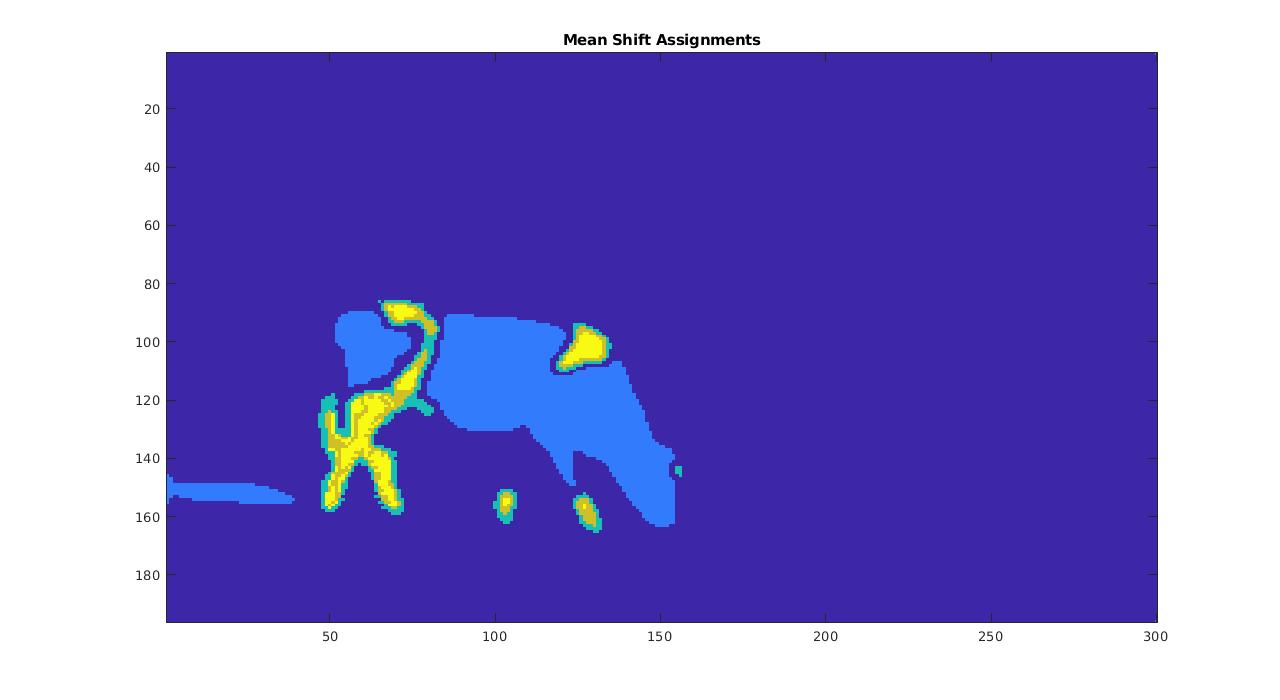
\includegraphics[width=\linewidth]{cow/ms_ass.jpg}
  \caption{Pixel Assigments}
\end{subfigure}%
\begin{subfigure}{.5\textwidth}
  \centering
  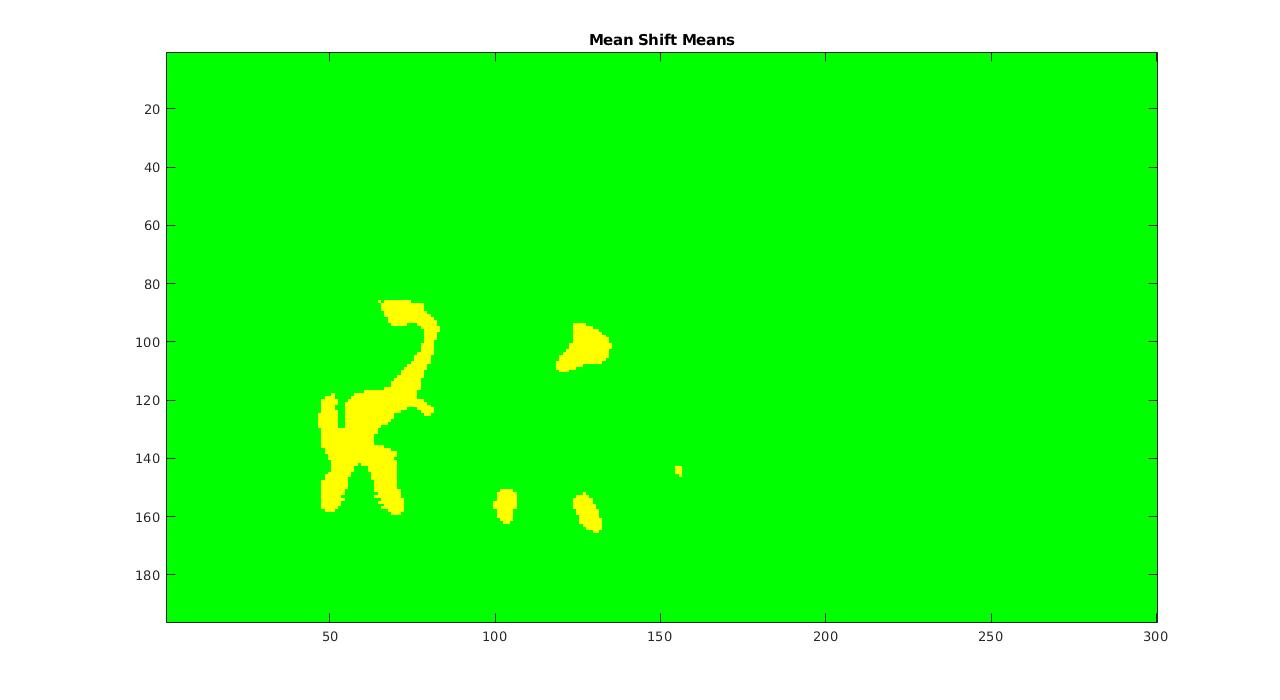
\includegraphics[width=\linewidth]{cow/ms_means.jpg}
  \caption{Cluster means}
\end{subfigure}
\caption{Cow image segmented with Mean-Shift (5 clusters found)}
\label{fig:ms_cow}
\end{figure}

\begin{figure}
\centering
\begin{subfigure}{.5\textwidth}
  \centering
  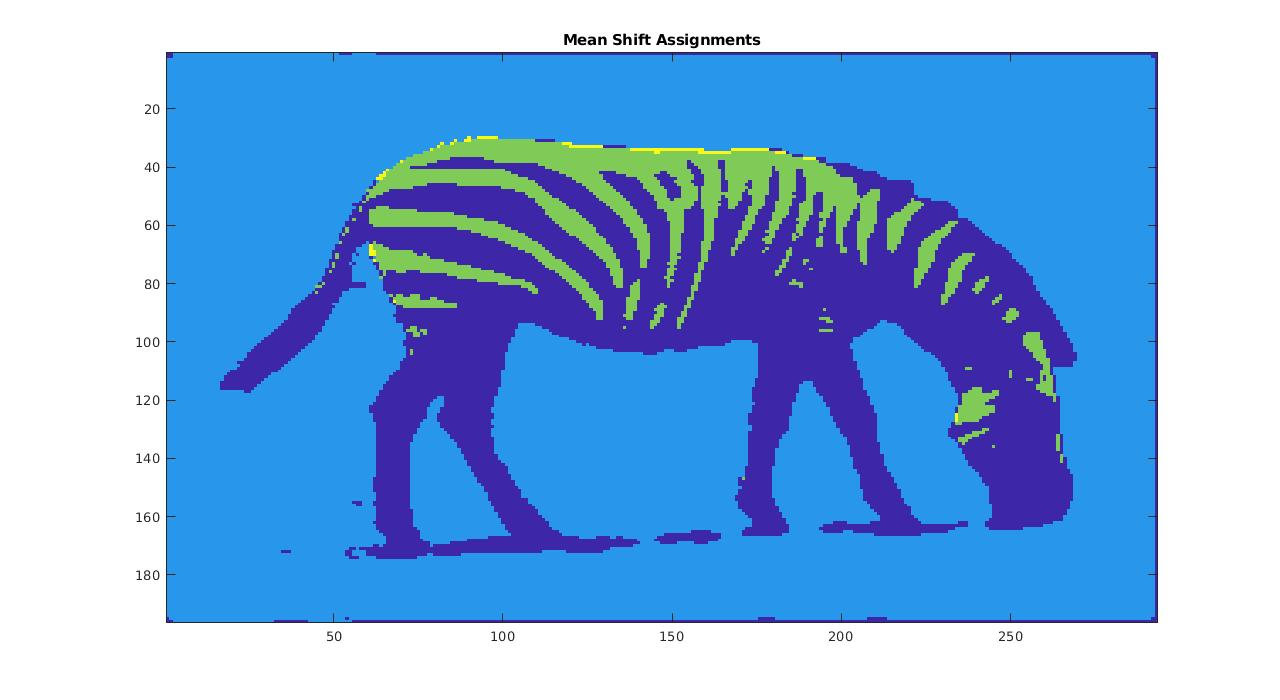
\includegraphics[width=\linewidth]{zebra/ms_ass.jpg}
  \caption{Pixel Assigments}
\end{subfigure}%
\begin{subfigure}{.5\textwidth}
  \centering
  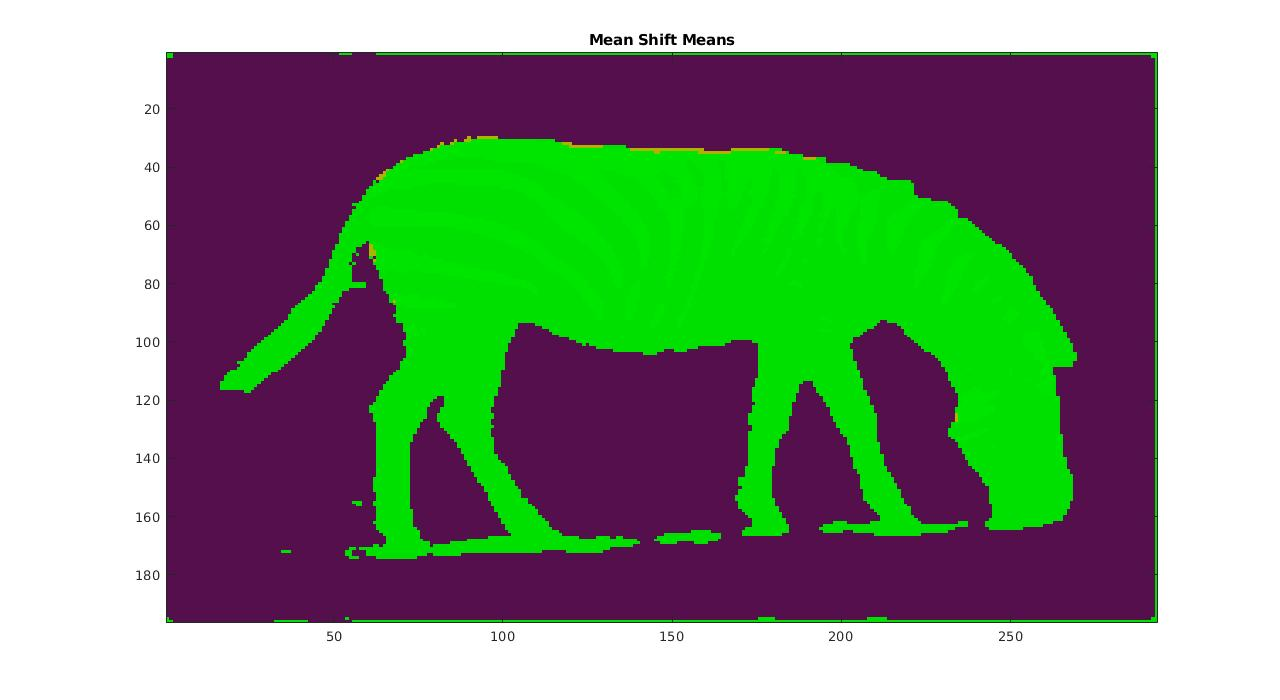
\includegraphics[width=\linewidth]{zebra/ms_means.jpg}
  \caption{Cluster means}
\end{subfigure}
\caption{Zebra image segmented with Mean-Shift (4 clusters found)}
\label{fig:ms_zebra}
\end{figure}


\section{EM Segmentation}

Before applying the EM I have normalized the pixels the same way as above. I have also initialized the means the same way as in k-means++ (this way the means will be probably far from each other and thus nicely distributed across the whole data set). Covariance matrix is initialized as described in the exercise slides. The algorithm always converged in less than 20 iterations and was very fast. The results for $K=3,4,5$ are displayed in Figures \ref{fig:em_cow} and \ref{fig:em_zebra}.


\begin{figure}
\centering
\begin{subfigure}{.3\textwidth}
  \centering
  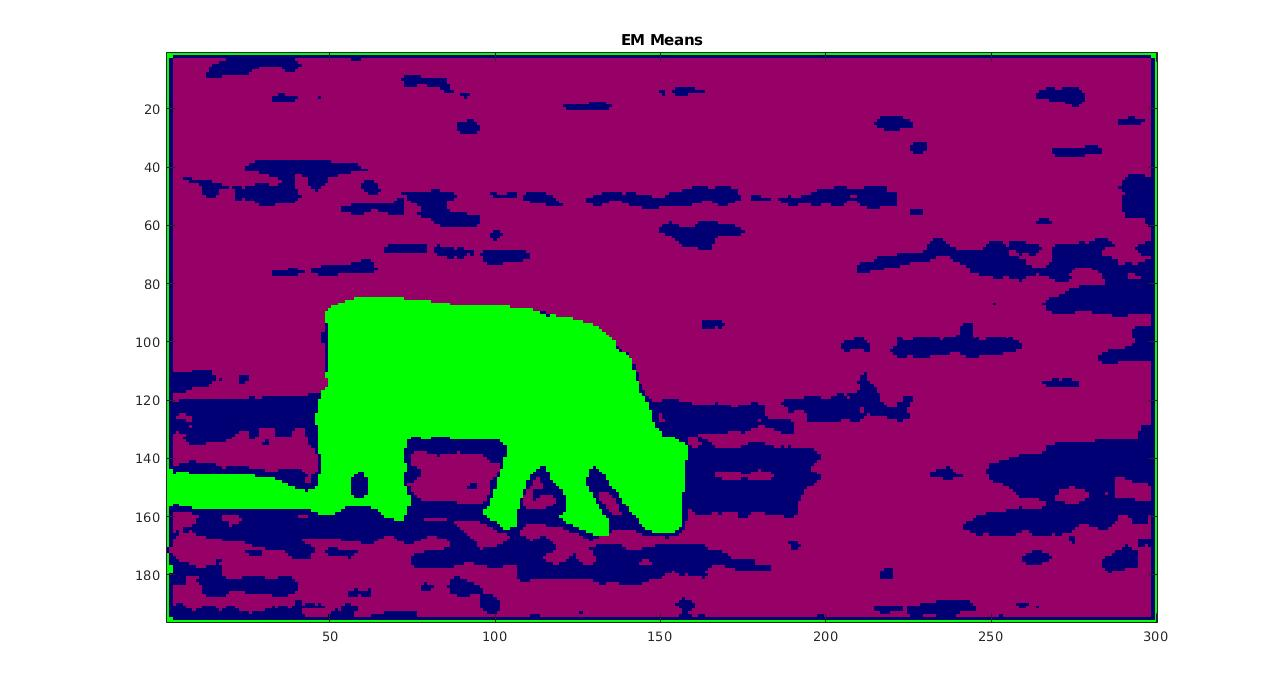
\includegraphics[width=\linewidth]{cow/em3_means.jpg}
  \caption{K = 3}
\end{subfigure}
\begin{subfigure}{.3\textwidth}
  \centering
  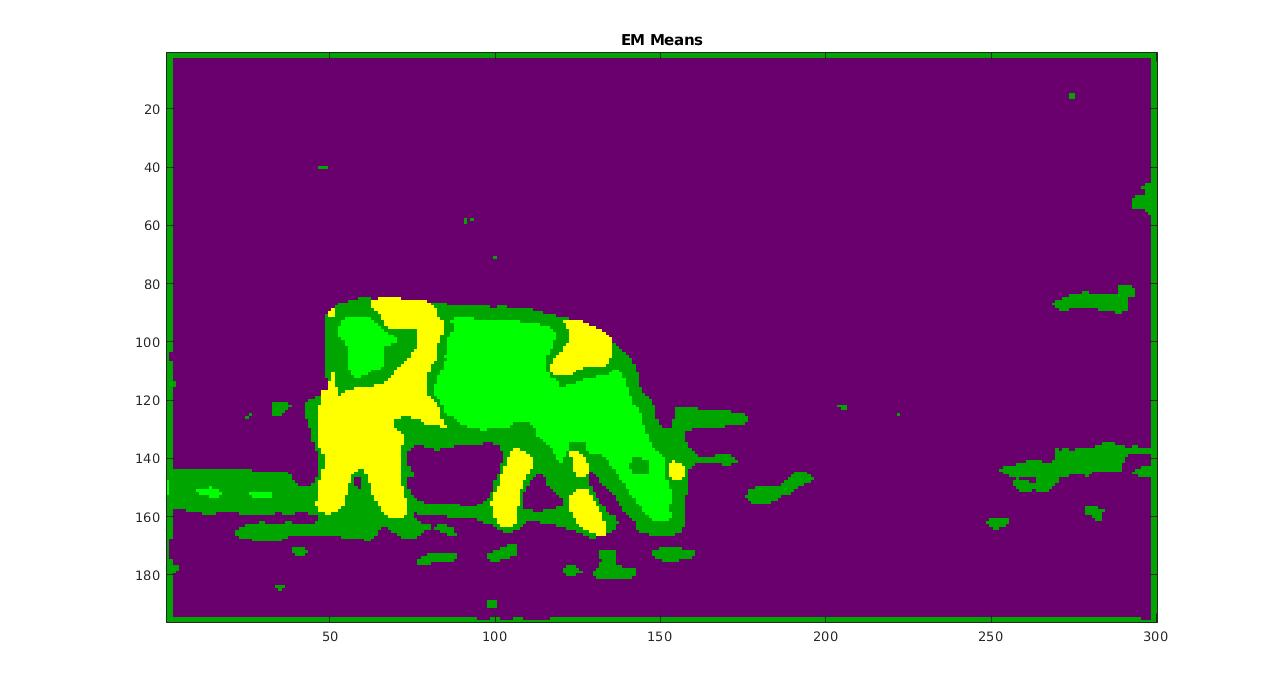
\includegraphics[width=\linewidth]{cow/em4_means.jpg}
  \caption{K = 4}
\end{subfigure}
\begin{subfigure}{.3\textwidth}
  \centering
  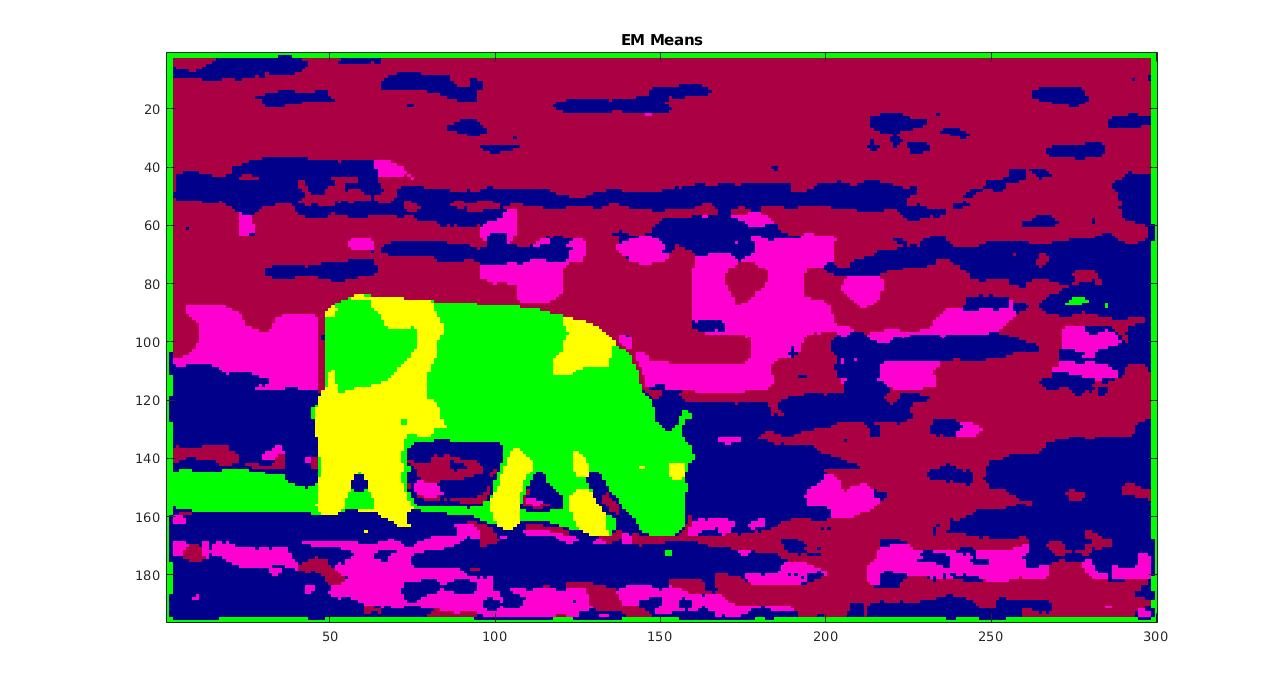
\includegraphics[width=\linewidth]{cow/em5_means.jpg}
  \caption{K = 5}
\end{subfigure}
\caption{Cow image segmented with EM (cluster means)}
\label{fig:em_cow}
\end{figure}

\begin{figure}
\centering
\begin{subfigure}{.3\textwidth}
  \centering
  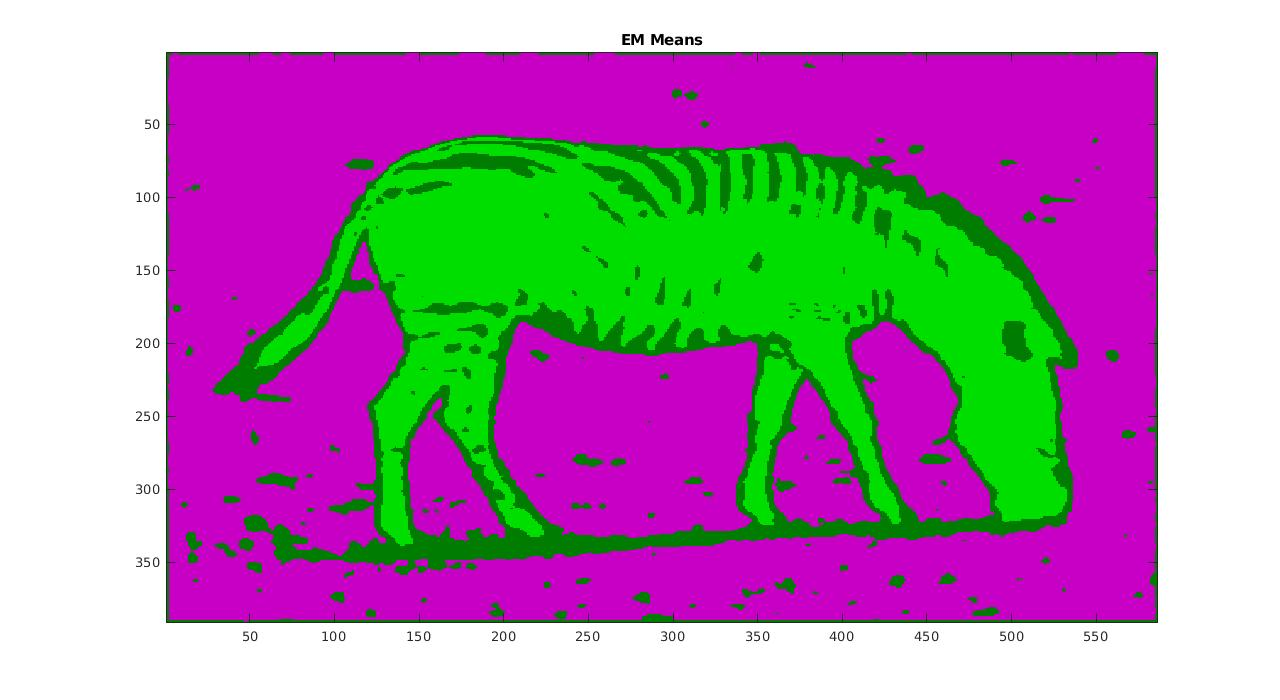
\includegraphics[width=\linewidth]{zebra/em3_means.jpg}
  \caption{K = 3}
\end{subfigure}
\begin{subfigure}{.3\textwidth}
  \centering
  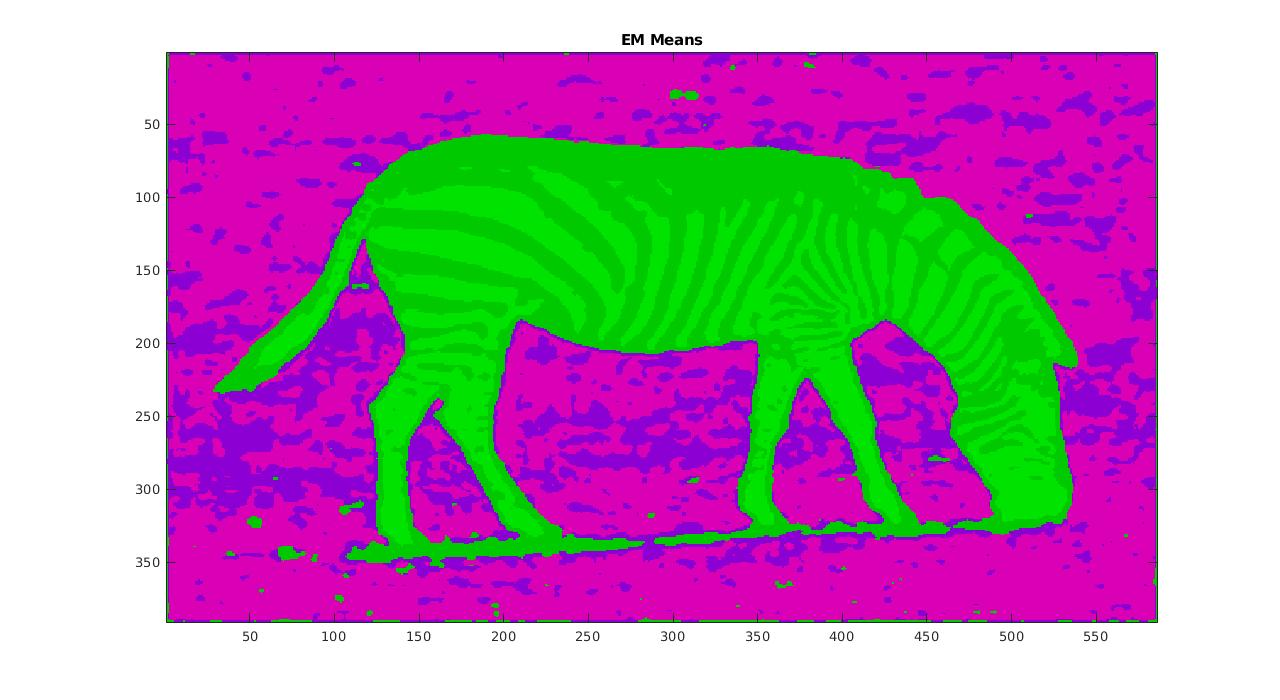
\includegraphics[width=\linewidth]{zebra/em4_means.jpg}
  \caption{K = 4}
\end{subfigure}
\begin{subfigure}{.3\textwidth}
  \centering
  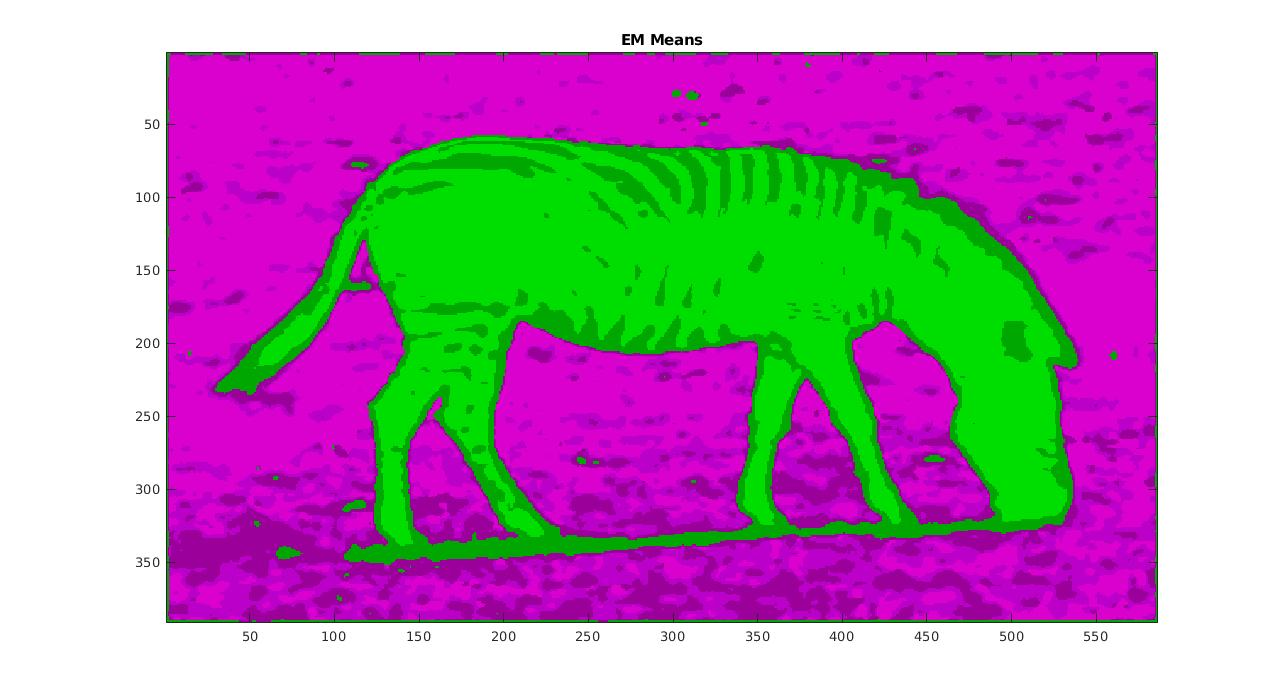
\includegraphics[width=\linewidth]{zebra/em5_means.jpg}
  \caption{K = 5}
\end{subfigure}
\caption{Zebra image segmented with EM (cluster means)}
\label{fig:em_zebra}
\end{figure}


\section{Results Discussion}

TODO: here put whatever....

\end{document}